\documentclass[11pt]{article}

\usepackage[margin=1in]{geometry}
\usepackage{booktabs}
\usepackage{graphicx}
\usepackage{amsmath}
\usepackage{array}
\usepackage{enumitem}

\setlength{\parskip}{0.5em}
\setlength{\parindent}{0pt}
\setlist[itemize]{leftmargin=1.5em, itemsep=0.2em, topsep=0.2em}

\title{Supplementary Material for\\
If You Hear It, Help Find It: Orthogonal Knowledge Distillation for Open-Vocabulary Audio-Visual Event Localization}
\author{Yi Xu$^*$, Cheng Chen$^*$, Wenzhuo Lei$^\dagger$\\
\small $^*$Equal contribution. $^\dagger$Corresponding author.\\
\small Tongji University, Shanghai, China}
\date{}

\begin{document}
\maketitle

This supplementary file is intended to be uploaded separately from the main paper. It collects implementation clarifications and qualitative evidence that were compressed out of the main submission for space.

\section{Protocol Clarifications}

We evaluate on \textbf{OV-AVEBench} using the official train/validation/test split of 13{,}182/5{,}798/5{,}820 samples. Each sample is treated as a query-conditioned temporal localization instance with 16 segments.

We report two metric groups because they answer different questions:
\begin{itemize}
    \item \textbf{F1@0.5} is the protocol-aligned metric used for direct comparison with the official fine-tuning baseline.
    \item \textbf{Segment AP/AUROC} are threshold-independent diagnostics that measure ranking quality under query-conditioned class imbalance.
\end{itemize}

Whenever we list AP/AUROC for the official baseline, those numbers come from re-scoring the released fine-tuning predictions under our segment-level ranking protocol rather than copying a number from the benchmark paper.

\section{Implementation Details}

\begin{table}[ht]
    \centering
    \caption{Implementation details for OV-OrthKD.}
    \label{tab:supp_impl}
    \begin{tabular}{@{}p{0.28\linewidth}p{0.65\linewidth}@{}}
        \toprule
        Item & Setting \\
        \midrule
        Video sampling & $224 \times 224$ inputs, 16 fps, 16 temporal segments per sample \\
        Audio sampling & 16 kHz waveform aligned to the same 16-segment timeline \\
        Student backbones & ConvNeXtV2-Tiny for vision and EfficientNetV2-B2 for audio \\
        Teacher backbones & InternVideo2 visual teacher, BEATs audio teacher, CLAP text encoder \\
        Fusion stack & Query-aware gate followed by a 4-layer temporal transformer, hidden size $D=384$ \\
        Projection heads & Three 2-layer MLP heads for visual-, audio-, and text-aligned student projections \\
        Optimization & AdamW, base learning rate $2 \times 10^{-4}$, \texttt{step400} schedule, early stopping \\
        Loss weights & $\lambda_{\mathrm{sup}}=1.0$, $\lambda_{\mathrm{text}}=0.8$, $\lambda_{v\text{-feat}}=0.4$, $\lambda_{a\text{-feat}}=0.1$, $\lambda_{\mathrm{orth}}=0.5$, $\lambda_{v\text{-kd}}=0.0$ \\
        Distillation mode & Teachers are frozen and exported offline; only the student is used at inference time \\
        Efficiency point & The main-paper latency and memory numbers are measured on a single RTX 5090 for one 16-segment clip \\
        \bottomrule
    \end{tabular}
\end{table}

\section{Additional Notes on Supervision Placement}

The strongest empirical pattern in the paper is not simply that more teachers help. The behavior is role-sensitive:
\begin{itemize}
    \item Strong visual transfer is useful on both the feature and diagnostic-logit sides.
    \item Weak audio transfer is useful only as an auxiliary representation constraint.
    \item Once weak audio is moved onto the decision path, performance drops sharply.
    \item Orthogonality helps only when it is paired with this asymmetric role assignment; by itself it is not a free gain.
\end{itemize}

This is why the paper frames the contribution as \emph{supervision placement} rather than generic multi-teacher distillation.

\section{Qualitative Case Studies}

Figure~\ref{fig:qualitative} shows representative qualitative examples. Each case compares temporal prediction curves from a student-only model, a decision-level KD baseline, and OV-OrthKD. The visual grids make the temporal evidence easy to inspect, while the curves show whether the model responds sharply at the correct event boundary.

\begin{figure}[ht]
    \centering
    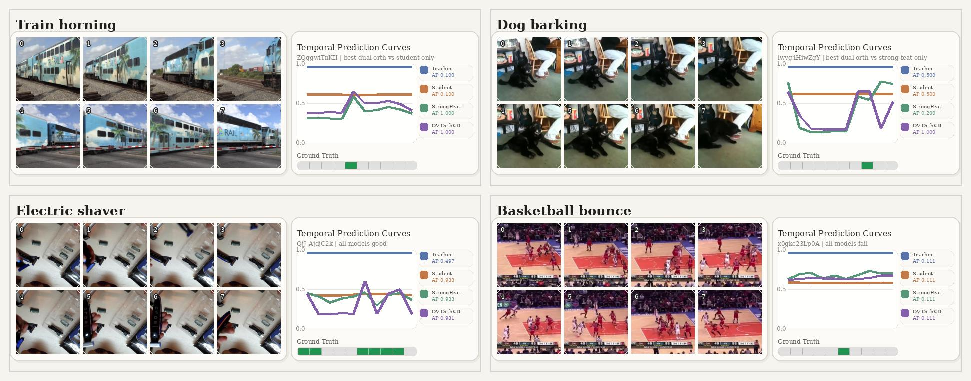
\includegraphics[width=\textwidth]{qualitative_contact_sheet.pdf}
    \caption{Qualitative comparison on four representative queries. In the train horn and dog barking examples, OV-OrthKD produces cleaner peaks around the correct event windows. In the electric shaver and basketball bounce cases, the auxiliary audio path improves semantic support without destabilizing the final boundary.}
    \label{fig:qualitative}
\end{figure}

\section{What Was Moved Out of the Main Paper}

For the main submission we kept only the evidence needed to support the central claim. The following items were intentionally moved to supplementary form:
\begin{itemize}
    \item protocol clarifications separating official F1 comparison from our ranking diagnostics,
    \item implementation details for the student/teacher interface and optimization recipe,
    \item qualitative comparisons illustrating the difference between feature-level help and decision-level distortion.
\end{itemize}

\end{document}
